\chapter{State of the Art}
\label{chap:state_art}
  
\epigraph{``\textit{Computer science is no more about computers than astronomy is
about telescopes.}''}{Edsger W. Dijkstra}
  
% Service oriented computing is at the origin of an evolution
% in the field of software development. An important challenge
% of service oriented development is to ensure the alignment
% between IT systems and the business logic. Thus, organizations
% are seeking for mechanisms to deal with the gap between
% the systems developed and business needs. The literature
% stresses the need for methodologies and techniques for
% service oriented analysis and design, claiming that they are
% the cornerstone in the development of meaningful services'
% based applications. In this context, some authors argue
% that the convergence of model-driven software development,
% service orientation and better techniques for documenting and
% improving business processes are the key to make real the idea
% of rapid, accurate development of software that serves, rather
% than dictates, software users' goals \cite{BichlerL06}.
 
Service oriented development methodologies providing
models, best practices, and reference architectures to build service-based
applications mainly address functional aspects \cite{sommerville08}. Non-functional aspects concerning services and applications semantics are often
expressed as requirements and constraints.
It is common that these aspects are not fully considered during the
development of applications. In many cases, they are considered once the
application has been implemented, in order to ensure some
level of reliability (e.g., data privacy, exception handling,
atomicity, data persistence). 
This situation leads to service-based
applications that are partially specified and that are
partially compliant with initial application requirements. 


In systems and requirements engineering, a non-functional
requirement (NFR) specifies criteria about the behaviour of a
system. These criteria may be not related to the results produced by the
system, but to other conditions of its performance and execution. 
Non-functional requirements are often called qualities of a system. 
They are also referred as ``constraints'', ``quality attributes'', ``quality goals'', ``quality of
service requirements'' or ``non-behavioural requirements'' \cite{Stellman2005}. 
In the case of service-based applications, non-functional requirements concern
the application itself as well as its component services. 

% For instance, by defining the
% correspondence between input and output data of the application.


% Non-functional requirements are related to business process associated to the
% behaviour of the application and in the case of service-based
% applications, they also concern the constraints imposed to the services. The
% plan for implementing functional requirements is detailed by the system design.
% The plan for implementing non-functional requirements is detailed by the system
% architecture. 

In the case of service-based applications, non-functional requirements concern
the application itself, as well as constraints imposed by the services. 
Associating non-functional requirements to services composition can help to
ensure that the resulting application is compliant to the user requirements and
also with the characteristics of the services it uses. As services are
independent components, ensuring non-functional properties is a challenge.   
%  in developing this type of application. To adapt quality properties in
% the web service development context can provide a greater software reuse.

  
%   Attempts to solve these problems have led to the development of a great deal of
%  work in non-functional attributes and non-functional requirements. 
%  
 Programming non-functional properties is not an easy task and different studies
\cite{Babamir2010,AgarwalLS09,CholletL09,GutierrezRF10,XiaoCZBOLH08,JeongCL09,Tsadimas:2012,Mairiza:2010}
 associate non-functional requirements and services using
different approaches. Although they are used as synonyms in most NFR approaches
\cite{Mairiza:2010}, we distinguish the concepts of non-functional requirements and non-functional attributes.
 NFRs are defined as a group of semantically correlated
 non-functional attributes (NFA). For example, \textit{security} is an
 non-functional requirement that comprises attributes such as
 \textit{confidentiality} and \textit{integrity}. A non-functional
 attribute describes the characteristics of a functional requirement
 \correctingText{\cite{RosaC04,MylopoulosBook99}}.
 
 This chapter \newText{\textit{(i)} presents the background concepts of this
 thesis,} \textit{(ii)} presents the state of the art of \correctingText{Web
 service} based methodologies and non-functional requirements for web service
 based applications, and \textit{(ii)} analyses the principal methodological
 concepts for web service development.
 

 
% The goal of this chapter is presents, based the concepts obtained from
% non-functional requirements and software engineering methodologies' works,
% a systematic analysis concerning \textit{(i) a towards NFR
% classification for reliable web service development, (ii) its application on the modeling web services composition and
% (iii) how to apply these set of concepts through a proposal for a reliable web
% service based methodology development}. 
 
 \correctingText{Considering the analysis, it} will be conducted through a
 systematic review\footnote{A systematic review provides means of identifying, evaluating, and interpreting the literature relevant to a particular research
 question or topic area~\cite{Kitchenham08}.} \cite{Kitchenham08}.
 The result of this review can be useful to summarize the existing evidence
 concerning a treatment or technology, to identify gaps in current research in
 order to suggest areas for further investigation, and to provide a background
 for new research activities. \correctingText{The bibliography will be analyzed in order to
 present the different existing concepts, proposals, problems and solutions
 related with each area.}
 
 \correctingText{The analysis is organized} in 2 parts to facilitate the
 understanding of the areas and related works and what their importance in the context of
 service-based development.  Our goal is to identify a common nomenclature for existing NFR
 and web service based methodologies and propose a specification of these
 concepts in the context of reliable web services development. 
 
 Since the focus of this work is the development of reliable service-based
   applications, we analyze \textit{what},\textit{where} and \textit{how}
   non-functional requirements are modeled in the development of this type of application. Allied to this,
   we analyze which methodologies address development of service-based
   applications and if they model non-functional aspects.
 
 This chapter is organized as follows. \newText{Section \ref{sec:background}
 presents the background concepts of this thesis, considering the following
 domains: model-driven development, service-oriented applications,
 non-functional requirements and design by contract.} Section \ref{sec:nfrs}
 presents the main concepts and works related with non-functional requirements for web service application. Section \ref{sec:metodologies} presents the main concepts and works related with methodologies for web service development. Section \ref{sec:classification} present a non-functional requirements model for 
 service-based development and a classification of the main terms used, divided
 into levels. Section \ref{sec:stateofart_conclusion} concludes for this
 chapter.


% The remainder of the Chapter is structured as follows: Apendix
% \ref{append:systematic_literature_review} shows what is an
% SLR is and describes the strategy's analisys for the state of the art's
% related works. The results of the SLR are analyzed in Section
% \ref{sec:results_systematic_literature_review}. We present the NFR meta-model
% and its application on reliable service modeling, and a proposal of NFR
% classification for reliable web service development in Section
% \ref{sec:proposal}. Finally our conclusions.
    
\newText{   
\section{Background}\label{sec:background}

The background of this work consists of the works addressing (i) model driven
development, (ii) service-oriented applications and (iii) non-functional
requirements. A number of approaches, models and solutions proposed in these domains were
studied, integrated and adapted for addressing the construction of service-oriented applications in the presence of non-functional requirements. We
underline in the following the key concepts that we used from each of the
domains of the background of our work.

\subsection{Model-Driven Development}

Model-driven development (MDD) approaches, specially the model-driven
architecture approaches provides a set of guidelines for the structuring of
specifications, which are expressed as models.

The MDA approach gives the facility to understand complex and real world systems
while providing an abstraction of the physical system. This  abstract view of
the system is represented through the OMG’s modeling standards namely the
Unified Modeling Language (UML) \cite{UML}, the Meta-Object Facility (MOF)
\cite{miller} and the  XML Metadata Interchange (XMI).

The Model-driven approach does not reinvent another software development process 
but it regroups the knowledge of software engineering concepts to express
architectures. The MDA approach is mainly based on the 
Model Driven Development (MDD) \cite{watson,miller} which suggests that a system
must be first modeled before it can be transformed to suit the final execution
platforms.

A MDA-based approach establishes a specific set of layers and transformations.
The Computational Independent Model (CIM), the Platform Independent Model (PIM)
and the  Platform Specific Model (PSM) are the three MDA model types.
Considering this concepts, a system can be expressed as the specification of an
execution environment for a set of models, the relationships between models,
meta-models and platforms. 

\paragraph{Computational Independent Model:} CIM is a view of a system without
any knowledge of the computation details. The aim of CIM is to link the needs of
the application client with the others models that are built in the next
development life cycle phases.

\paragraph{Platform Independent Model:} PIM is a view of a system without any knowledge of the 
implementation details. The PIM model requires that model elements contain enough 
information to represent the system independent of platform.

\paragraph{Computational Specific Model:} PSM is a view of a system with
specific knowledge of the implementation platform. After the platform
independent model has been accurately defined, the platform specific details can
be handled in the PSM. 


 Another important aspect of the MDA approach is the transformation between 
models. Models transformation relies on a set of mapping rules between models
that inform the transformer tool about the patterns it needs to follow to output
the target model. Then, consistency and validation of models can be automated
during this transformation process, improving the efficiency of
generated applications.

\subsection{Service-Oriented Applications}

Service-Oriented Applications are defined based on the Service-Oriented
Architecture (SOA) \cite{2,Rosen08,somf} paradigm for organizing and use of
distributed computing resources that may be under the control of different domains, providing a uniform meaning for discovery, interaction and
use of these resources. SOA is a set of principles and methodologies for
designing and developing software in the form of interoperable services. 

he use of SOA makes possible the integration of applications that are web based and
make use of multiple platforms for its implementation. SOA also defines a
interface in terms of protocols and functionality.
 
As an architecture, SOA relies on principles of service-orientation (Web
services). This is motivated by the hypothesis that, if a service provides a
simple interface that abstracts its complexity, users can access the services independently, without
know the development platform on which it was implemented.
So, service-orientation requires loose coupling of services with operating
systems and other technologies that underlie applications.

Web Services can be defined as software that can be discovered and invoked
through the Web. Normally independent and self descriptive, several initiatives
related to web services have been implemented with the intention of providing
platforms and languages that allow easy integration of heterogeneous systems.
Services are usually built from the following specifications: XML,
SOAP~\cite{soap}, WSDL~\cite{wsdl}, and UDDI~\cite{uddi}. Besides these, it is
possible to use other technologies for services, such as ontologies
DAML-S~\cite{Liu04} that define standards for discovery, description and
invocation of services. An example of another initiative that uses service-oriented technology is the Business Process Execution Language for Web Service (BPEL4WS) \cite{bpel,bpmn,bpm}, where a composition of web services
can be described through representation of business processes.

Considering composition of services in
general, two paradigms guide the compositions: the
choreography and orchestration \cite{SBS04}.
The orchestration is concerned with the flow of interactions between services
(business logic and execution order of services, such as a workflow). 
The orchestration requires an  engine that coordinates the composition
execution. The choreography describes the order in which messages are ordered
for using the methods exported by one or several services. The choreography is
used for expressing the conversations that an application can have with a
service. A conversation specifies the sequence of valid messages that a service
con receive. These sequences correspond to the protocols for exchanging messages
with a service. 
 

\subsection{Non-Functional Requirements}

A non-functional requirement (NFR) is a requirement that specifies criteria that
can be used to judge the operation of a system, rather than specific behaviors.
Non-functional requirements are often called qualities of a system.
However, for \cite{MylopoulosBook99} there is not a formal definition or a
complete list of non-functional requirements. NFRs are classified into consumer-oriented and
technically-oriented attributes \cite{MylopoulosCN92}. 
  

Based on \cite{MylopoulosCN92}, during the design process goals are decomposed
design alternatives are analyzed with respect to their tradeoff design
decisions are rationalized goal achievement is evaluated and a selection is made In this
approach NFR-related knowledge is codied into methods and correlation rules.
This way a body of codied NFR-related knowledge offers the needed subject
matter and vocabulary and is made available and reusable throughout the
process \cite{Chung91}.

In the area of software requirements, the term non-functional requirements has 
been used to refer to concerns not related to the functionality of the software.
However, different authors characterize this difference in informal and unequal 
definitions, such as ``\textit{Requirements which are not specifically concerned with
the functionality of a system. They place restrictions on the product being developed and the 
development process, and they specify external constraints that the product 
must meet}'' \cite{Chung2009}.

Expressing and enforcing non-functional properties for distributed systems is a
well-known problem with  several associated existing solutions that have modeled
thoroughly  them for providing middleware services. For example in object
oriented solutions  like CORBA, and component oriented solutions like EJB.
Models and protocols have been defined in the distributed systems and the
database domains for dealing with non-functional requirements that concern for
example, security , tolerance to failure (e.g, transaction monitors,
synchronization protocols like 2PC), persistence. Lately service-oriented
applications, call for approaches that can include these aspects trying to be
loyal to the facility of construction philosophy. Some solutions leave this task
to the middleware infrastructure (e.g., the service bus petals
\footnote{http://petals.ow2.org} offers some non-functional services), to the
engines that execute them. Other approaches like \cite{Derks:2001}  include the code
that implements non-functional properties, as protocols within the coordination
code  that implements the application logic of service-oriented applications or
within the communication protocol used for calling services methods (e.g. data
encryption of SOAP messages). This later approach is particular to works
stemming from the Business Process domain (BPM  \cite{bpmn}) and also to WS-*
standards. 

\subsection{Design by Contract}

 We used the notion of reliability in order to have a common approach for dealing
with non-functional requirements (i.e., ensuring that the system respects them
and defining actions when they are not respected). The concept of reliability of
service-oriented applications used in our work is associated to the concepts of
{\it correctness}, {\it robustness} and {\it reliability} introduced in (i)
\textit{Design by Contract} \cite{Meyer92,MeyerN93,Meyer97}, (ii) referred by
\cite{Meyer92,Meyer97} and (iii) defined in the database domain.

Design by Contract is a method for developing software. Design by Contract is
the principle by which interfaces between software modules should be designed
using precise specifications. The principle behind Design by Contract is a class
and its client have a contract with each other. Contracts define mutual benefits
and obligations (pre-conditions and post-conditions, respectively), and
constraints (invariant). Contracts are defined in program code through comments
of their own programming language and is translated into executable code by the
compiler. The properties (predicates) of the contract are known as assertions
(assertions). 

Assertions are representations of states. Expressions are true at certain points
of a code \cite{Meyer92}, becomes important when one wants to prove the correctness
a program. To be able to prove the correctness of a given program
or a piece of code, it is necessary to define logical expressions that represent
desired states. If one of the conditions is not satisfied, there was something
wrong with either, the defined assertion or the definition of the program.   


\textit{Design by Contract} defines reliability as a concern that integrates the
ability of a software element to perform the tasks as defined in its
specification (correctness) and that reacts appropriately to abnormal conditions
(robustness). Furthermore,  the notion of contract proposed by
\cite{Meyer92,MeyerN93,Meyer97} enables the specification of actions to take
when one of these properties is not respected by a service.
\cite{Meyer92,Meyer97} associate the notion of reliability to the conformance
between the requirements specification of a software component and its
implementation with the objectives to avoid possible bugs. Thus, reliability is
associated to the absence of bugs of a software component with respect to its
specification (during the design phase).      
 
 In the database domain, reliability is often related to a kind of failure
 tolerance in the sense that a database application is reliable if it handles
 exception and it ensures that data consistency will be maintained despite
 possible physical and logic failures \cite{Adiba:1981,MartinAD92}.

}

\bigskip

\correctingText{

Based on this background concepts, the challenge was to analyze
approaches concerning the non-functional properties and generalize them into the
meta-models that are core components for a service-oriented methodology.
 
}

\section{Non-Functional Requirements for Service-Based Applications}   
\label{sec:nfrs}   

This section presents a systematic review of the non-func\-tion\-al
requirements and properties used in the context of service-oriented
development. The purpose of our analysis is:
\begin{itemize}
  \item to identify the concepts, properties and notations used in the
  service-based systems development;
  \item to find if there is any pattern or relationship between non-functional
requirement concepts in different modelling levels.
\end{itemize}

The functional and non-functional requirements are refined in each phase of the
development. As a result, the granularity of the requirement becomes tiner and
more precise.

% For each phase of the development, the requirements and non-functional
% requirements are refined. As a result of this process, the granularity of the
% concepts described by the requirement becomes thinner and more precise. 

% The focus of a modeling-based non-functional requirements becomes important
% because it reveals a continuing need on the development of distributed
% service-oriented. Thus, it is necessary identify how non-functional requirements
% are classified in different development process phases and iterations.

% Thus, this section also presents the collected data and results
% from the research work analysis according to some research questions. Once the
% sources' extraction execution had been completed, it was important to be sure
% that multiple publications of the same approach were not included in the data analysis. Tables \ref{tab:result02}
% and \ref{tab:result03} show the results of each work under each question
% described in section \ref{subsec:question}.  





% % Among the properties presented we highlight the security
% % and performance properties. All users want to access data
% % securely and quickly. Most studies analyzed have both properties. Reliability is
% % also an important non-functional requirement presented in some papers and needed
% % to end users. 

% 
% The analisys was carried out by effectuating the following activities:
% \textit{(i) question formulation; (ii) source selection; (iii) selection
% process; (iv) information extraction;} and \textit{(v) results}.

We propose 7 research questions ($RQ_1$ to $RQ_7$) to guide our analysis of the
bibliography about non-functional requirements. 
For each question we define a set of possible answers in order to guide
the analysis.
These possible answers are defined from our knowledge on each topic. 
The questions are closely related to service-oriented development with a NFR focus.
They are:
\begin{itemize} 
  \item \textbf{\texttt{$RQ_1$:}} \correctingText{How are NFR modelled by existing
  methodologies for developing Web services applications?}
  \begin{itemize}
	  \item \textit{Answer is specific to each proposal}
	\end{itemize}  
 \item \textbf{\texttt{$RQ_2$:}}\correctingText{ Which are the NFR that are more frequently
 used by developing web services?}
 	\begin{itemize}
	  \item \textit{Possible answers: security / availability / portability / \ldots / reliability /
	  performance}
	\end{itemize}
  \item \textbf{\texttt{$RQ_3$:}} What is the software
  development approach used in the work?
	\begin{itemize}
	  \item Possible answers: \textit{Model driven approach (*MDD) / Ontology (*Ont) / Formal method
	  (*FM) / Artificial intelligence (*AI) / Business Process Modeling (*BP)
	  Traditional (*TDT)}
	\end{itemize} 
  \item \textbf{\texttt{$RQ_4$\footnote{\newText{Since the objective of our work was
  to develop a methodology for supporting the service-oriented application development process,  the  goal of RQ$_4$ was to
look for a ``standard'' or a classification of non-functional requirements  for
service-oriented development. As any research question, it can be too particular
and can leave some works outside its scope (e.g., KAOS \cite{UszokBJ04} and
i-star \cite{Yu97} were not part of the result).}}:}} 
  \correctingText{What is the discipline of the ``\textit{non-functional requirements}'' /
  ``\textit{non-functional properties}'' used in the work?}
  \begin{itemize}
	  \item Possible answers: \textit{Software architecture / QoS model / Language definition /
	  Methodology / etc}
	\end{itemize}	
  \item \textbf{\texttt{$RQ_5$:}} Does the paper propose a (meta)model
  describing and analyzing NFR? Is there any relationship between
  the proposed non-functional requirements (meta)model and business
  services\footnote{\newText{Note that the term business services is used to make the difference between the services that participate in
the implementation of an application logic from the services used for
implementing non-functional aspects. For instance, CORBA domain services are
those equivalent to  business services. BPMN \cite{bpmn} defines a similar term
called \textit{Service operation}  that is part of the business process.}}? 
\begin{itemize}
	  \item Possible answers: \textit{yes / no} -- \textit{yes / no}
	\end{itemize}  
  \item \textbf{\texttt{$RQ_6$:}} Are the non-functional aspects treated in
  an independent way?
\begin{itemize}
	  \item Possible answers: \textit{single / composition}
	\end{itemize}
\item \textbf{\texttt{$RQ_7$:}} Which is the publication year of the paper?
	\begin{itemize}
	  \item Possible answers: \textit{Year of publication}
	\end{itemize}	   
\end{itemize}


% \subsection{Source Analysis}
% \label{subsec:souce_analysis}

% In the development of systems, for each phase of development,
% the requirements are being refined and the granularity becomes tiner after each
% iteration. With the analysis, we can identify how these NFRs have been
% classified.
 
The research questions identify characteristics
 of the ser\-vice-oriented application development, especially the
modelling of non-functional requirements/properties, how they are addressed and
if they are classified.  
 
% The focus of a modeling based on non-functional requirements becomes important
% because it reveals a continuing need on the development of distributed
% service-oriented. Among the properties presented we highlight the security
% and performance properties. All users want to access data
% securely and quickly. Most studies analyzed have both properties. Reliability is
% also an important non-functional requirement presented in some papers and needed
% to end users.
 
% Based on the first research question, the results were the most different
% possible. Despite being different, the nomenclatures in each paper  most often are
% associated to the same concept. The question was, ``\textit{How NFR are modeled
% in existing methodologies for reliable web services development?}'' We will
% highlight the nomenclature used for each work.

 
\subsection{Concepts and Works}
\label{subsec:nfr_concepts}

In order to classify the available works using the research questions, we
proceed with a systematic selection of the published papers in our field of
interest.

We used the approach described in Appendix \ref{append:analysis} for searching,
collecting and selecting some works related with non-functional requirements for
developing service-based applications. This approach selects published articles
from known sources, \newText{such as \textit{IEEE, ACM} and \textit{Science
Direct},} to be considered for inclusion in our study. Based on these data we analyzed concepts used in each work for the description of NFRs and the
differences between them. The notation used to refer non-functional
requirements will be highlighted in \textit{italic}, including the set of values
that can be associated to each concept. For example, a notation used by a work
can be \textit{quality property} or \textit{non-functional concern}, and the values associated with
its notation are \textit{security}, \textit{reliability}, \textit{transaction},
etc. Thus, considering each research question, we analyze a set of works in
order to identify any pattern or divergence between the analyzed literature. 

% Each work will be analyzed according to their proposal and the described
% questions.   

\bigskip
\bigskip

Babamir et al.\cite{Babamir2010} ranks services \textit{quality properties}
in three categories (business level, service level, system level).
\textit{Quality properties} are associated with \textit{quality constraints},
that are defined as assertions or propositional logic formulas.
\textit{Non-functional attributes, composition model entity} and \textit{model entity} are the notations used by
Xiao et al. \cite{XiaoCZBOLH08} for classifying the different concepts for
non-functional requirements modeling. Non-functional attributes (NFAs) describe
the \correctingText{non-functional} aspects in the abstract process models. The
framework to model NFRs proposes to annotate composition models with NFAs.

D'Ambrogio \cite{DAmbrogio06} uses the term \textit{quality characteristics}
to group similar characteristics into \textit{quality categories}. Each
\textit{quality characteristic} is quantified by \textit{quality dimensions}.
\textit{Quality characteristic} is a quantified QoS aspect, for example
\textit{latency, throughput, reliability, availability}, etc. \textit{Quality
characteristics} of a common subject are grouped into abstract \textit{quality
categories}, for example \textit{performance} (for latency and throughput characteristics) and
\textit{dependability} (for reliability and availability characteristics).  
 
The terms \textit{category, sub-category}
and \textit{property}  are used by Yeom
et al.\cite{Yeom2006} to classify non-functional requirements.
\textit{Business}, \textit{service} and \textit{system} are the possible values to be associated
with the proposed terms, and a \textit{sub-category} can be \textit{security,
value, interoperability}, etc. The work in \cite{Yeom2006} defines a \textit{web
services quality model}, which considers non-functional properties in several
aspects. In this model, web services qualities are classified in categories and
sub-categories. Chollet et al.\cite{CholletL09} uses only two terms to
classify and relate quality properties with services, they are:
\textit{activity} and \textit{quality property}. Each activity represents a
functional property that can be divided in sub-activities, depending on its
granularity. For non-functional requirements, the work in \cite{CholletL09}
describes the possibility of creating different meta-models for each
\textit{quality property}, and then relate them with activities.   


Schmeling et al.\cite{SchmelingCM11} uses the 
\textit{non-functional concerns (NFC)} notation to describe NFRs. This term
encompasses two aspects: the specification of NFCs and their realization.
\cite{SchmelingCM11} defines that a \textit{functional concern (FC)} is a
consistent piece of functionality that is part of a software system.
\textit{Non-functional concern (NFC)} is a general term describing a matter of interest or importance that does correspond
to a non-functional requirement of a system, for example, \textit{security,
reliability, transactional behavior}, etc. A \textit{non-functional action} represents some
behavior that results in a \textit{non-functional attribute}. An example of
\textit{non-functional action} is \textit{encryption}, which realizes the \textit{non-functional attribute},
\textit{confidentiality}. A \textit{non-functional activity} is also used as a
term, which means to encapsulate the control flow of \textit{non-functional
action} that apply to the same subject. The term is used in analogy to activity
and action in UML2 \correctingText{\cite{SchmelingCM11}}.

Ceri et al.\cite{CeriDMF07} uses the terms \textit{policy, rule,
condition} and \textit{action model} to specify NFRs, and in a similar way,
Agarwal et al.\cite{AgarwalLS09} also uses the concept of \textit{service
policy} associated with the concept of service. Each service is also associated
with a \textit{service property}, which may have a specific value
(\textit{security, reliability}, and so on). Each service is also associated
with a \textit{unit function}, that represents one or more
requirements.

Ovaska et al.\cite{OvaskaEHPA10} uses
\textit{quality attribute, category, conceptual layer} and \textit{importance}
to organize and classify the NFRs, Pastrana et al.\cite{PastranaPK11} uses
the term \textit{contract} to describe non-functional requirements. In a
\textit{contract} it is possible to define pre-conditions, post-conditions and
invariants. A \textit{web service} can have many \textit{contracts}, that
defines many \textit{assertions} and are associated with \textit{quality
properties}. 




Some related papers do not have any
nomenclature to classify non-functional requirements. However, some of them uses
the \textit{attribute} notation \cite{ZhangPSP05,BasinDL06,JeongCL09}, other
use \textit{properties} \cite{Fabra2011}, \textit{factors}
\cite{MohantyRP10,GutierrezRF10}, \textit{characteristics}
\cite{DiamadopoulouMPS08}, \textit{quality level} \cite{ModicaTV09} or
\textit{values} \cite{ThissenW06,BasinDL06}.

%  However, none of them present a
% specific notation or model to classify non-functional requirements.


\subsection{Analysis}
\label{sec:proposal}

% The purpose of this analysis is to identify the properties and non-functional
% requirements used in the development of systems, looking for patterns
% or relationships between non-functional concepts in different
% modeling levels.

Although there exist many different types of notation used for classifying
non-functional requirements, in general, the values associated to them are the
same, \textit{i.e.} \textit{security, performance, reliability, usability, availability}, etc. What
distinguishes the different approaches is the adoption of different NFR
hierarchies in order to prioritize or classify the quality requirements. Another interesting factor
is that each work uses different approaches to model these requirements.
Thus, there are different kinds of notations for non-functional
requirements.
 
A number of approaches use
\cite{DAmbrogio06,CholletL09,SchmelingCM11,BasinDL06,Fabra2011,OvaskaEHPA10} MDD
(Model Driven Development) for designing and developing systems. Fabra
\textit{et al.} \cite{Fabra2011} presents a complete methodology that does not
focus on non-functional requirements. Fabra \textit{et al.} \cite{Fabra2011}
describes the importance of the use of MDD in the development of service-oriented applications. \cite{ThissenW06,ZhangPSP05} use formal methods to define a development process based on NFR for web services,
\cite{AgarwalLS09,PastranaPK11} use ontologies for the definitions and
modeling of non-functional requirements and \cite{XiaoCZBOLH08,GutierrezRF10} use Business Process Modeling (BPM) for
system specification, including NFR. Most works focus on composition
service modeling while others define requirements models for representing the
properties they use.

In \cite{Babamir2010,Yeom2006} non-functional properties for web services
are classified into three views such as
\textit{service level, system level} and \textit{business level}.
In the \textit{\textit{business}} level the quality properties are:
\textit{service charge, compensation rate, penalty rate} and
\textit{reputation}; at the \textit{\textit{service}} level the quality
properties are: \textit{performance} and \textit{stability}; and at the
\textit{system} level the quality properties are classified into:
\textit{manageability, interoperability, business processing} and
\textit{security}.

In the method defined in \cite{XiaoCZBOLH08}, each task in the process model is
annotated with the NFAs (\textit{non-functional attributes}). During the design phase, the
service composition and the definition of NFAs are separated. Then,
each task in the process model is annotated with the corresponding NFA. The
attributes are related with tasks or data item. For data, the NFAs are:
\textit{value} and \textit{range}; and for tasks the NFAs are: \textit{cost,
time, resources} and \textit{expression}.

D'Ambrogio \cite{DAmbrogio06} presents a WSDL extension for describing the QoS
of web services. The process is based on MDA. The work presents a catalog
of \textit{QoS characteristics} for the web service domain and the Q-WSDL
(Quality WSDL) meta-model for modeling QoS properties in web services. The properties
presented are: \textit{availability, reliability} and \textit{access
control}. \cite{CholletL09} presents a security meta-model for web service
composition. The non-functional requirements considered are
\textit{authentication, integrity} and \textit{confidentiality}. Each property is related with a service activity. In \cite{SchmelingCM11}, authors
present an approach and a toolset for specifying and implementing the
composition of several non-functional properties of Web services. The
non-functional attributes described in \cite{SchmelingCM11} are: \textit{confidentiality, integrity
(security concern)} and \textit{response time (performance concern)}.

The work presented in \cite{ThissenW06} describes
steps to design a selection mechanism of services identified as candidates for
participating in a composition, considering their quality properties. The steps
are: \textit{(i)} identification of relevant QoS information; \textit{(ii)} identification of basic composition patterns and
QoS aggregation rules for these patterns; and \textit{(iii)} definition of a
selection mechanism of service candidates. As QoS properties considered in
\cite{ThissenW06} are: \textit{performance, cost, reliability} and
\textit{availability}. 
  
% We highlight the following works: \cite{CeriDMF07, 
% Yeom2006,JeongCL09,PastranaPK11}. These research works present a relevant
% detail of some NFR and a good detail of them in each stage of development.

Among the properties presented we highlight \textit{security}
and \textit{performance}. Users usually need to access data
securely and quickly. Most studies have both properties as the most
important non-functional requirements. \textit{Reliability} is also an important
non-functional requirement presented in some works and required by end users.

We can now relate the research questions presented in section \ref{sec:nfrs},
with the works described above. Tables \ref{tab:result02} and \ref{tab:result03}
show the results.

The vocabulary used for naming and characterizing NFR is not stable, 5 works out
360 (1.6\%). 19 of the total of works chosen (26.31\%) propose a
classification of non-functional requirements (see appendix
\ref{append:analysis}).

% The many different types of NFR terms used
% in these works, there is still no clear classification of NFRs
% and a hierarchy or dependency between them. Only 5 of the works present a hierarchy
% among the different non-functional requirement notations, representing only
% 1.6\% of the total (over 306 works - appendix \ref{append:analysis}) and 26.31\% of total of
% works chosen (over 19 works - appendix \ref{append:analysis}). This hierarchy
% is used according to the modeling level and process phase. 

% Among these works, we highlight
% \cite{Yeom2006,DAmbrogio06,CeriDMF07}, because it presents the types of NFR and
% their importance at each modeling level.

  
\begin{table}[ht!]
\centering
\scriptsize
\begin{tabular}{l|l|l|c|l}
  \hline 
  \hline
   \textbf{Reference} & $RQ_1:$ \textbf{\textit{NFR concepts}} &
   $RQ_2:$ \textbf{\textit{NFR values}} & $RQ_3:$ \textbf{\textit{Approach}} &
   $RQ_4:$ \textbf{\textit{Domain / Scope}} 
   \\
  \hline
  \hline  
  Babamir et al. \cite{Babamir2010} &  property / & responsiveness /
  availability   & TDT & Software architecture
 \\  
  & category /  & performance / sla properties   &  & 
 \\
 &  constraint &    &  & 
 \\ 
  \hline   
 
  Yeom et al. \cite{Yeom2006} & category / & business value / performance /
   & TDT & QoS model\\ 
   & sub-category / & stability /manageability /   & & \\
   & property & security / business processing  & & \\
    &  & interoperability & & \\ 
  \hline 
  
  Xiao et al. \cite{XiaoCZBOLH08} &  NF attribute  & time /
cost / resource  & BP  & Business processes
   \\
 	&   &   &  & modeling
   \\   
  \hline 
  D'Ambrogio \cite{DAmbrogio06} &  characteristics /  & availability /
  reliability / & MDD & WSDL \\ &  category /  &  access control  &  &
  extension
  \\
  &  dimension &    &  & 
 \\
   \hline
  Chollet et al. \cite{CholletL09} & activity / & security  & MDD 
  & Orchestration Framework
   \\
  &  NF attribute &    &  & 
  \\
  
  \hline
  Schmeling et al. \cite{SchmelingCM11} & NF concern / & security &
  MDD &  Web service 
  \\
  & NF attribute / &  &
   & composition process
    \\
  &  NF action / &    &  &
   \\
  &  NF activity	 &    &  &
  \\ 
  \hline
    Thi{\ss}en et al. \cite{ThissenW06} & NF value  &  performance /
  reliability &  FM & Software architecture \\  
   & & cost / availability &  & \\  
  \hline
  Zhang et al. \cite{ZhangPSP05} & attribute /& security & FM &  Access control 
   \\
  &  predicate &    &  &
  \\
  
  \hline
  Basin et al. \cite{BasinDL06} &  attribute & security  & MDD & System
  architecture
  \\
  \hline
  Ceri et al. \cite{CeriDMF07} & police / rule  & n.a. & TDT & Context-aware
  applications
   \\
  &  condition / action &    &  &
  
  \\
  \hline
  Fabra et al. \cite{Fabra2011} & property & storage /
  processing & MDD & Web service methodology 
  \\
   &   & (*case study) &  & 
  \\
  \hline
  Modica et al. \cite{ModicaTV09} & quality level & sla
  properties & TDT &  Service oriented 
  \\
   &  &  &  & architecture \\
  \hline
  Ovaska et al. \cite{OvaskaEHPA10} & attribute & security / reliability
  & MDD &  Model development
  \\
   
  &  category &    &  &
  \\
  \hline
  Agarwa et al. \cite{AgarwalLS09} & property / & \textit{not explicitly
  defined} & Ont & Policy language
  \\
   
  &  policy / &    &  &
  \\
  
  &  function &    &  &
  \\
  \hline
   &  & operation cost /&  &  \\
  &  & performance / availability /  &  &  \\
  Jeong et al. \cite{JeongCL09} & NF attribute & accessibility / security /
  & AI  & Service oriented   \\ 
   &  &
  interoperability / usability / & & \\ &  & user satisfaction &  & architecture
  \\
  \hline
   &  & performance / reliability /  &  & \\
   & NF property / & scalability / capacity /&  & \\
  Pastrana et al. \cite{PastranaPK11} & contract  / & robustness /
  precision / & Ont & Web service methodology\\
  & assertion / & accessibility
  / availability / &  & \\ 
   & NF behaviour & interoperability / security  &  & \\    
  \hline
  Diamadopoulou et al. \cite{DiamadopoulouMPS08} & NF characteristic &
  user' subjective & TDT & Web service selection  \\ 
   &  & perception  & &  \\
  \hline
  Gutierrez et al. \cite{GutierrezRF10} & NF factor & Security  & BP &  Web
  service
  \\
   &  NF sub-factor&   &  &  development process
  \\  
  \hline
  Mohanty et al. \cite{MohantyRP10} & NF attribute or & reliability /
  performance / & & Artificial intelligent /\\ 
  & NF factor & integrity / usability  & AI  & Web services classification	 \\
  &  & response time / documentation &   &  \\
  
  \hline  
  \hline  
\end{tabular} 
\caption{Research question results - $RQ_1$, $RQ_2$, $RQ_3$, $RQ_4$.}
\label{tab:result02}
\end{table} 
 
\begin{table}[ht!]
\centering
\scriptsize
\begin{tabular}{l|c|l|c}
  \hline 
  \hline
   \textbf{Reference} & $RQ_5:$ \textbf{\textit{Service model}} --
   \textbf{\textit{Business services}} &
$RQ_6:$ \textbf{\textit{Service type}} &   $RQ_7:$ \textbf{\textit{Year of publication}} 
   \\
  \hline
  \hline  
  Babamir et al. \cite{Babamir2010} & no -- yes  & composition & 2010   
 \\  
  \hline   
  Yeom et al. \cite{Yeom2006} & yes -- yes & single   & 2006  \\  \hline
  Xiao et al. \cite{XiaoCZBOLH08} & no -- no & composition    & 2008
   \\ 
  \hline 
  D'Ambrogio \cite{DAmbrogio06} & yes  -- no & composition  & 2006 \\
   \hline
  Chollet et al. \cite{CholletL09} & yes -- yes & composition  &  2009 \\
  \hline 
  Schmeling et al. \cite{SchmelingCM11} & no -- no & composition &  2011 \\ 
  \hline
   Thi{\ss}en et al. \cite{ThissenW06} & no -- yes & composition & 2006
   \\
  \hline
  Zhang et al. \cite{ZhangPSP05} & no -- no  & single  & 2005 \\ 
  \hline
  Basin et al. \cite{BasinDL06} & yes -- no & single / composition  & 
  2006\\
  \hline 
  Ceri et al. \cite{CeriDMF07} & no -- no  & single  &  2007\\ 
  \hline 
  Fabra et al. \cite{Fabra2011} & yes -- yes & composition  &  2011\\
  \hline
  Modica et al. \cite{ModicaTV09} & no -- no & composition & 2009\\ 
  \hline
  Ovaska et al. \cite{OvaskaEHPA10} & yes -- no & single & 2010\\
  \hline
  Agarwa et al. \cite{AgarwalLS09} & yes -- no & single / composition  &  
  2009\\
  \hline
  Jeong et al. \cite{JeongCL09} & no -- no  & composition &  2009\\
  \hline
  Pastrana et al. \cite{PastranaPK11} & yes -- no & composition &  2011 \\
  \hline
  Diamadopoulou et al. \cite{DiamadopoulouMPS08} & no -- no & composition 
  & 2008\\
  \hline
  Gutierrez et al. \cite{GutierrezRF10} & no -- no &  single / composition 
  & 2010\\
  \hline
  Mohanty et al. \cite{MohantyRP10} & no -- no  & single  & 2010\\
  \hline
  \hline  
\end{tabular}
\caption{Research question results - $RQ_5$, $RQ_6$, $RQ_7$.}
\label{tab:result03}
\end{table} 

There are other works
\cite{ieee_1998,CysneirosLN01,Cleland-HuangSZS06,Glinz05rethinkingthe,sommerville08}
that consider and propose non-functional requirements classifications. A number
of software attributes are defined as requirements in
\cite{sommerville08,ieee_1998}. According to \cite{ieee_1998}, the most common
non-functional properties are: \textit{performance}; interface; operational;
resource; verification; acceptance; \textit{maintainability}; documentation;
\textit{security}; \textit{portability}; quality; \textit{reliability};
\textit{usability}; and \textit{safety}. We \textit{highlight} those that are
used in most analyzed classifications. \cite{ieee_1998} proposes an NFR specification
and a template for specifying requirements, considering both, functional and
non-functional properties.

The NFRs are classified in 4 main concepts by \cite{CysneirosLN01}. The
classification uses \textit{quality properties}. These properties are:
\textit{performance; security; cost;} and \textit{usability}. Pastrana
\cite{PastranaPK11} describes an ontology based methodology and uses a NFR
classification based in some properties, most already described in other works.
However that work is the only one to use \textit{scalability, capacity}
and \textit{precision} properties. Considering web services development,
these properties are not very frequently used, however, considering data
processing, these properties can be important in cases of large data processing
requests through services.

Sommerville \cite{sommerville08} classifies requirements,
either functional or non-functional, in three main blocks:
\textit{process, product} and \textit{external}. \cite{sommerville08} 
also defines a sub-classification considering the system domain.
Software requirements are classified as: \textit{usability, reliability, safety,
efficiency, performance} and \textit{capacity}.  
   

% Based on the works presented in \cite{Cleland-HuangSZS06,Glinz05rethinkingthe},
% and considering the previous analysis of NFR, the properties highlighted are
% security, performance and reliability. Although the works have
% different focuses and the NFR classification and definition are made in
% accordance with different arguments, the more present in NFR ratings
% requirements are that ones presented in Figures \ref{fig:NRFmodel} and
% \ref{fig:proposalNRF}.


Some requirements may determine the system design, for example, \textit{(i)}
keep certain functions in separate modules; \textit{(ii)} check data integrity
for critical variables; and \textit{(iii)} permit only limited communication
(requester / provider), are examples of restrictive requirements
\cite{ieee_1998}. These examples are related with some NFR concepts as: \textit{security, reliability} and
\textit{availability}. 

% Thus, in the context of service-based
% development, it is important that non-functional requirements are described
% through abstract modeling levels.
 
%    Thus, based on theses works and the
% results obteined in the systematic review, the results presented in tables
% \ref{tab:result02} and \ref{tab:result03}, we will propose a NFR model and
% classification for service based application development.
   
% \subsection{NFR Metamodel:} 
% \label{sec:servicedefinitionNFR} 


In the service-based development there is a clear difference between the
business, service and system levels. Quality requirements are treated
differently in each of these levels. Despite the different nomenclatures, they
can be described in general as \textit{non-functional concerns/requirements} and
\textit{non-functional attributes}.
  
%Considering \cite{ieee_1998} and \cite{sommerville08}, we notice that
Restrictions are usually related to use cases and functional requirements
(\cite{ieee_1998} and \cite{sommerville08}), and in most cases, a service
activity can be represented as an use case. This is the way in which
non-functional requirements are related with web services. They do not propose a
specific way for designing services constraints, they assume that a service is
modeled as a use case, and it has quality requirements.

At the service level, each service activity is related in some way with the
concept of contract. Contracts can be grouped into policies and their
rules. Policies are directly related to concepts like quality,
security, performance and availability; contracts are associated with non-functional attributes. 

\bigskip
\bigskip

Due to the variety of tools and new approaches for web service development,
there is not (yet) a consensus on a software process methodology for web
services
\cite{PapazoglouH06,Papazoglou03,Milanovic2006,MilanovicM06,FeuerlichtM05,Ramollari_asurvey,somet2005}.
%  In order to develop and use such a methodology, it is of paramount importance to
% provide adequate descriptions of its expected capabilities and competences.  
 
Works proposing methodologies can be
classified into two types: (\textit{i}) those that propose new approaches for non-functional
properties guarantees; and (\textit{ii}) those proposing service-oriented
development methodologies for the whole development process.
    
\cite{HL05TACoS} proposes \textit{Design by Contract} for web services. It is
possible to describe three levels for specifying contracts: \textit{implementation level,
XML level} and \textit{model level}. Design by Contract applied to web services
addresses the verification of web services through runtime checkers,
before the deployment, such as \textit{jmlrac} \cite{LeavensCCRC02}, by adding behavioral
information to the specification of services, using JML \cite{LeavensCCRC02}.

CDL (\textit{Contract Definition Language}) \cite{Milanovic2006} is a XML-based
description language, for describing contracts for services. The
development with CDL offers an architecture framework, design standards and a
methodology \cite{MilanovicM05,Milanovic05,Milanovic06,MilanovicM06}, that can
be easily understood and applied to the development of applications. The
greatest difficulty is that the language only
represents contracts for services. Its specification is generated by
refining B \cite{AbrialLNSS91} machines that describe
the services and their compositions. 

% Papazoglou \textit{et al} \cite{PapazoglouH06} propose a methodologie that is
% based on the SOA extension. This work defines a service
% oriented business process development methodology with phases for business process
% development. The whole life-cycle is based on six phases, they are: planning, analysis and design,
% construction and testing, provisioning, deployment, and execution
% and monitoring. This proposal has as focus only the development
% phase and does not define specific development models, however
% describes the activities sequence needed to services develop.
% 
% IBM proposes a methodology for the development of SOA
% solutions, called SOMA \cite{soma}. SOMA defines a life-cycle with seven
% phases: business modelling and transformation, solution management, identification,
% specification, realization, implementation and deployment monitoring
% and management.To assist the SOMA development is necessary to use the tools
% proposed by IBM, which makes the process very expensive for the dependence of
% these tools. 

% Unlike the analysis of works presented in this section, 
% we propose a meta-model for NFR modeling and a NFR classification
% (business, service and system modeling levels) for reliable service-based
% development.


\section{Methodologies for Service Oriented Development}
\label{sec:metodologies}


In this section, we present an analysis of some methodologies for
service-oriented development. We defined 5 research questions to guide our analysis. The questions are closely related to service-based
systems. The criteria used for evaluation and comparison are:


% , which will be described highlighting its key features, as well as
% their contributions and limitations when used in a development process. 




\begin{itemize} 

 \item \textbf{\texttt{$RQ_8$:}} What is the scope of the methodology?
 	\begin{itemize}
	  \item \textit{This item will review the major phases and
  the purpose of each particular phase in the context of the project and
  service-oriented development.}
	\end{itemize}
  \item \textbf{\texttt{$RQ_9$:}} 
  How does the methodology define the development process according to the
  adopted notation?
  \begin{itemize}
	  \item \textit{This item describes which notation is used by the methodology
	  for designing its models, e.g., MDA, UML, SysML, etc.}
	\end{itemize}	
  \item \textbf{\texttt{$RQ_{10}$:}} Does the methodology use a formalism?
  If so, What is the formalism used for specifying services? 
\begin{itemize}
	  \item \textit{ The purpose of this item is to determine whether the
	  methodology proposes the use of a formalism for specifying
  the services, their compositions and iterations.}
	\end{itemize}  
  \item \textbf{\texttt{$RQ_{11}$:}} What is the approach for describing
  services?
\begin{itemize}
	  \item \textit{ The purpose of this item is to determine the approach
	  adopted by the methodology for describing the development process.}
	\end{itemize}
	  \item \textbf{\texttt{$RQ_{12}$:}} Which models does the methodology
	  propose?
	  \item \newText{\textbf{\texttt{$RQ_{13}$:}}Does the methodology defines
	  service's choreography or service's orchestration?} 
	\begin{itemize}
	  \item \textit{This item discusses the models proposed by
  methodologies for specifying the system behavior and modeling
  high-level business requirements.}
	\end{itemize} 
\end{itemize}


% \begin{enumerate}
%   \item \textbf{\textit{Methodology's scope:}} This item will review the
%   proposed scope of the analyzed methodologies, which is the major phases and
%   what is the purpose of each particular phase in the context of the project and
%   service-oriented development.
%   \item \textbf{\textit{Proposed models:}} Each development methodologies
%   analyzed defines a set of models for the design of
%   information system. This item discusses the proposed models by each
%   methodologies for the specification of system behavior and modeling of
%   high-level business.    
%   \item \textbf{\textit{Modeling notation:}} There are several notations and
%   diagrams that can be used to describe applications. This item describes which
%   notation is used by the methodology for the design of its
%   models, \textit{e.g.} MDA, UML, SysML, etc.
%   \item \textbf{\textit{Formalism used for service specification:}} In this item
%   is analyzed if the methodology proposes the use of any formalism to specify
%   the services, their compositions and iterations.
%   \item \textbf{\textit{What is the approach to service description?:}} In this
%   section analyzes how the various methodologies build and deploy services and
%   their compositions. Thus, the aim is to highlight the differences in the
%   systems developing processes in each analized approach.     
% \end{enumerate}  

Along with the research questions, we also compared the MDA models 
proposed by different methodologies. 

In general, for service-based systems, there is no specific method to conduct
the development process. Our analysis, helped us to identify how these methodologies define activities and models to design reliable
services, as well as service-based applications.

\subsection{Concepts and Works}
\label{subsec:methodology_concepts}

Over the last few years, a number of approaches have been proposed for the
development of web services. These approaches range from the proposal of new languages for web service
descriptions~\cite{bpel03, MPC08, wscl02, Martin04,SBS04} to techniques to
support phases of the development cycle of this kind of
software~\cite{lipari2007,BianculliGSBG07}. In general, the objective of these
approaches is to solve specific problems, like supporting transactions or
QoS, in order to improve the security and reliability service-based
applications. Some proposals address service composition: workflow
definition~\cite{AalstHKB03,MuP06} or semantic equivalence between
services~\cite{BHM06}. The proposed solutions come from many communities, including those of Theoretical Computer Science~\cite{SBS04,VA05,HamadiB03,AlH01,GGP08}, Software
Engineering~\cite{burdy:05,AalstHKB03,Aal03,choreoWG,MendesPDB09}, Programming
Languages~\cite{MPC08,bpel03} and Databases~\cite{PiresBM02,ABM01}.
However, in spite of the variety of tools, there is not (yet) a consensus on a software
process methodology for web services. 

\newText{Considering the composition of services in
general, two paradigms guide the compositions: the
choreography and orchestration \cite{SBS04}.
The orchestration is concerned with the flow of interactions between services
(business logic and execution order of services, such as a workflow). 
The orchestration requires an  engine that coordinates the composition
execution. The choreography describes the order in which messages are ordered
for using the methods exported by one or several services. The choreography is
used for expressing the conversations that an application can have with a
service. A conversation specifies the sequence of valid messages that a service
con receive. These sequences correspond to the protocols for exchanging messages
with a service.}

% In order to develop and use such a
% methodology, it is of paramount importance to provide adequate descriptions of
% its expected capabilities and competences.

% New proposals for web technology such as XML, web services, business process
% management and semantic web have promoted an evolution of
% techniques and  extensions for web based development. Thus, 

There are methodologies that address the service-based development towards a
standard or a new way to develop reliable service-based applications. The
methodologies analyzed in this work are: SOD-M \cite{valeriaThesis} and SOMF
\cite{somf} representing the model based development for web services; S-Cube
\cite{scube2010book} representing the business processes and service-based
development; SOMA \cite{soma} that is a methodology described by IBM
for SOA solutions; Extended SOA \cite{PapazoglouH06} merges RUP\cite{rup} and
BPM\cite{bpm} concepts for service modeling; DEVISE \cite{DEVISE} is a
methodology for building service-based infrastructure for collaborative
enterprises. Furthermore, there are other proposals, such as the WIED
model \cite{TongrungrojanaL04} that acts as a bridge between business modeling and
design models. Also, traditional approaches for software engineering
\cite{sommerville08} are being applied to service development.

\bigskip

\textbf{SOD-M:} Service-Oriented Development Method \cite{CastroMV11}
proposes a service-oriented approach and model-based development for web systems.
SOD-M proposes models and standards primarily focusing on the
development of the systems behavioral characteristics, setting standards for
the construction of business models at a high-level of abstraction. The approach
describes three  meta-models organized according to the MDA (\textit{Model
Driven Architecture}) ~\cite{miller} architecture levels: CIM (\textit{Computational
Independent Models}), PIM (\textit{Platform Independent Models}) and PSM
(\textit{Platform Specific Models}).

At the CIM level, 2 models are defined: \textit{value model}
~\cite{Gordijn02valuebased} and \textit{BPMN model};
At the PIM and PSM levels, DSL models for service. The
PIM-level models are: \textit{use case, extended use case, service process} and
\textit{service composition}. The PSM level models are: \textit{web
service interface}, \textit{extended composition service} and \textit{business
logic}. 


The methodology provides a framework for the development of
service-oriented applications with models that can express the whole
development process of services-based applications. However, SOD-M
has no support for describing and modelling non-functional requirements. 

% There is no component model that could express the property of non-functional
% requirements, such as security, performance or availability of services.


The basis of SOD-M is a set of concepts guiding the whole
development, including transformations between models. The concepts are
represented through a meta-model. This meta-model describes concepts of both the
business and system views.
 
% The \textit{value model} is a business model that describes a business case as
% a set of values and value activities shared by business actors. The
% \textit{BPMN model} (business process model) is used to describe the business
% process related to the environment which the system will run. These two models
% represent the independent aspects of computing and they are described in the
% more abstract modeling level. The \textit{use case model} is used to represent
% the business services to be implemented by the system, while the \textit{extended use case model} is a
% behavioral model, to represent the system features as a way to implement
% the business services. The \textit{service process model} describes the set of
% activities that must be performed on the system to implement a business service.
% Finally, the \textit{service composition model} represents the full flow of
% business system. This model is an extension of the service process model,
% however, in more detail.

In SOD-M, the PIM level models the entire structure of the application flow,
while, the PSM level provides transformations towards more specific platforms.

The methodology provides model transformations among:
\textit{CIM-to-PIM, PIM-to-PIM} and \textit{PIM-to-PSM} transformations. Given
an abstract model at the CIM level, it is possible to apply transformations for
generating a model of the PSM level. In this context, it is necessary to
follow the process activities described by the methodology. The model to model
transformations are defined using ATL \cite{atl_manual}.

SOD-M defines a set of concepts according to two points of view:
\textit{(i)} \textit{business}, focusing on the characteristics and requirements
of the organization and \textit{(ii)} \textit{system requirements}, focusing on
features and processes to be implemented in order application requirements. In
this way, SOD-M aims to simplify the design of service-oriented applications, as
well as its implementation using current technologies.

% \begin{figure}[ht]  
% \centering
% 
% \includegraphics[width=0.8\textwidth]{figs/sodmConcepts.png}
% 
% \caption{SOD-M Concepts Meta-model\cite{CastroMV11}.} 
% \label{fig:sodmConcepts}
% \end{figure}



\bigskip

\textbf{S-Cube:} The S-Cube Framework \cite{scube2010book} proposes an
integrated structure for developing service-based applications. S-Cube offers
three areas: \textit{Business Process Management, Composition and Coordination
of Services; and Infrastructure}. These areas are the backbone of the framework
that are directly linked to three other areas for supporting systems
development: \textit{Engineering and Software Design; Monitoring; and Security
and Software Quality}. 

The methodology aims to guide the development of applications and describes
some essential activities, such as \textit{(i) description of business objectives},
\textit{(ii) domain assumptions defining}, which are
pre-conditions to be met for a particular application domain, \textit{(iii)
description of domains}, and \textit{(iv) description of scenarios for
each domain}.

The S-Cube methodology does not provide an exhaustive list of rules for
describing services. The S-Cube framework provides activities in various
service-oriented development areas, however, it is still required to apply its
concepts in real case studies to give an idea of its application, given the fact
that its structure is very complex and multidisciplinary.


\bigskip

\textbf{DEVISE:}  \cite{DEVISE} identifies issues to
be considered in service-based design, and gives generic guidelines for
addressing them. DEVISE helps the developer in the design of new applications
as a collection of web services, and provides means of porting existing
applications to services-based platforms.

\newText{DEVISE \cite{DEVISE} is a methodology for defining infrastructure Web
services and prescribes adherence to a thought process that entails the division
of the design of a Web Services based collaborative application.}

\bigskip

\textbf{SOMA:} \textit{Service-Oriented Modeling and Architecture} \cite{soma}
is a methodology by IBM for SOA solutions. SOMA defines a seven-phase
development life-cycle: \textit{business modeling and transformation; management
solution, identification, specification, realization, implementation}, and
\textit{monitoring of implementation and management}.

At each stage, different tasks are carefully defined,
such as the definition of business architecture, development of service model,
specification of services, etc. 

% \begin{figure}[ht]  
% \centering
% 
% \includegraphics[width=0.8\textwidth]{figs/soma.png}
% 
% \caption{SOMA Methodology Structure \cite{soma}.}
% \label{fig:soma} 
% \end{figure}

The SOMA conceptual model is based on the SOA architectural style it
defines an interaction model with three main parts: (i) \textit{the service
provider} (which publishes a service description and provides the implementation for the
service); (ii) \textit{consumer services} (which can use the URI for the service
description directly or can find the service description in a service registry
for the call); and the (iii) \textit{service broker} (which provides and
maintains a record of services).

SOMA proposes the use of IBM Rational platform for SOA developing, and other
different IBM tools that are available to analysts, software architects and
application developers. 

% This tool is perhaps the biggest disadvantage of
% applying the IBM proposal, because of the need to use different types
% of tools such as IBM WebSphere and Rational Software, all of them very
% complex in order to develop applications. 

\bigskip

\textbf{SOMF:} \textit{Service-Oriented Modeling Framework} \cite{somf} is a 
model oriented methodology for modeling software with the best practices of
software project activities and different architectural setting. SOMF can be
used to describe enterprise architectures, service-oriented architecture (SOA)
and cloud computing. SOMF offers a variety of modeling practices and disciplines
that can contribute to developing a successful service-oriented applications. 
The main goals of SOMF are \cite{somf}:
      

% The SOMF structure offers a technology independent notation, focusing on
% development-based services. Model concerns the construction of a abstract representation of
% a software product, application, software component, system, or any other software asset. 

\begin{enumerate}
%   \item No prior knowledge of programming language or modeling tools are needed;
%   \item Modeling activities are fast. Models and diagrams can be developed in
%   minutes;
  \item A methodology describes SOMF modeling
  activities and each model transformation;
%   \item Model oriented. SOFM describes eight models transformations
%   for development of applications;
%   \item Flexible design to provide an easy development of models;
  \item The diagrams are created obeying some project
  patterns.
\end{enumerate}

The methodology's model transformations in SOMF aim to
describe and refine aspects in the system development
process. The models are: \textit{discovery model, analysis model, design model,
architectural model, implementation model, quality model, operations model,
business model, governance model}. 

% These models are integrated into each
% methodology activity and in their respective phases. For service modeling, SOFM
% highlights the need of:
% 
% \begin{enumerate}
% \item Identify service relationships;
% \item  Establish message routes between consumers and providers
% services;
% \item  Provide efficient service orchestration and choreography methods;
% \item  Create service transaction and behavioral patterns;
% \item Providing solutions for deployment of services.
% \end{enumerate}

% The main disadvantage of SOMF is the use of its own modeling notation, 
% different from those existing service notations. The methodology introduces
% several new concepts and notations for modeling services and compositions during the
% development phases. Along with SOMA, SOMF also focus on models to represent all
% aspects of the application.

\bigskip

\textbf{Extended-SOA:} \cite{PapazoglouH06} adopts the lifecycle
of web development services focussing on the \textit{analysis, design}
and \textit{development} phases, with approaches that are centered in
functional requirements.  According to \cite{PapazoglouH06}, a specific
methodology for developing services-based is important to specify, build, improve and customize business processes available on the Web. 

Extended SOA has a hierarchical structure for the development of web
services, where layers are defined as follows: \textit{Business (Service)
Domain, Business Processes, Business Services, Infrastructure Services,
Component-based Service Realizations} and \textit{Operational Systems}.

The methodology is partly based on other successful models and
related development, such as the Rational Unified Process (RUP),
Components-based development and Business Process Modeling (BPM). The difference
with those models is that Extended SOA life cycle focuses specifically on
service-oriented development.

Extended SOA is based on three principles for the design and development of
services, they are: \textit{Service coupling, Cohesion of service}
and \textit{Service granularity}.

Considering service-oriented projects, it is preferable to create high-level
interfaces with coarse granularity to implement a complete business process,
since multiple calls of service increases network traffic.
As the services are in a cooperative environment, it is unfeasible to create
services with finer granularity. It is preferable to create functions with
finer granularity in a local environment. Thus, the methodology aim is to
achieve services integration and interoperability. The Extended SOA phases are:
\textit{Planning, Analysis, Design, Implementation, Testing,
Provisioning, Implementation, Execution} and \textit{Monitor}.

% \textbf{Planning:} The planning phase determines the
% viability, nature and scope of service solution. The planning
% phase is very similar in software development methodologies, including RUP. The
% key requirement at this stage is to understand the business environment and make
% sure that all necessary controls are incorporated into the project to a
% service-oriented solution.
% 
% \textbf{Analysis:} The analysis phase examines the server-side existing
% services to understand which processes/services that already exist and what
% need to be created and implemented. 
% 
% \textbf{Design:} The service specification is a set of three
% elements of the specification, all equally important:
% \textit{structural specification, behavioral specification} and
% \textit{business specification}.
% 
% \textbf{Implementation:} The methodology implementation phase includes
% Web services development, from the service interface description to the service
% implementation definition. The methodology does not present anything new to this
% phase in the development of services web.
% 
% \textbf{Test:} The methodology proposes the conventional testing approaches,
% such as \textit{test functional, performace test, dynamic test} and
% \textit{integration test}. However, the methodology concludes that
% \textit{dynamic test} approach is more appropriate to be used to web service
% test.

\bigskip
\textbf{Traditional Software Engineering Approach:} Sommerville
\cite{sommerville08} proposes a general approach for the development of applications that use web services. Its
structure uses the activities of design, development, construction and testing of web services and their
compositions. The proposal is based on the traditional concepts of software
engineering, such as:
 
\begin{itemize}
  \item Software reuse: standards-based web service that provides a mechanism
  for inter-organizational computing;
  \item Use process engineering services to produce reusable web services;
  \item Perform composition of services to facilitate and improve the
  development of applications;
  \item Show how business process models can be used for the design of
  service-oriented systems.
\end{itemize}

% Existing approaches to software engineering have to involve the concept of
% web services for software development. 
Service engineering allows the development of reliable and
reusable services. Thus the entire development life cycle focusses on the
reuse of independent services. 

% With this development we have software \textit{reuse}. On the other hand there is the development with services. The development of
% dependable software where services are the key components. By this
% way we have the  software development \textit{with reuse}.

% A key difference between a service and a component is that services are
% independent \cite{sommerville08}. Components are always used with another
% software component. The services come with a message-based communication, and these messages expressed
% in XML, which are independent. Thus, the definition of a method must be based on
% a set of principles to be followed for the development of
% applications that use web services and their compositions.

A service must be designed as a abstraction that can be reused by different
systems. The main activities for service engineering are: \textit{(i)}
Identification of candidate services; \textit{(ii)} Service design; and
\textit{(iii)} Service implementation.

% From the identification of system requirements, the whole project is based
% on services that can be reused or implemented. From this
% identification, the project is developed in order to be implemented the
% services needed in the application. If the service is already available,
% adapt it to current system needs.



%*********************************************************************************************************
\subsection{Analysis}
\label{sec:methodology_analisys}
%*********************************************************************************************************

Our analysis is based on the research questions 8 to 12  described at the
beginning of this section. Table \ref{tab:method_analysis}
summarizes of the main features of the methodologies described above,
considering the research questions.

% The questions attempt to cover important aspects of
% service-oriented application development. We analyze the
% aspects of modeling and models proposed, which
% notations are used for modeling, and what is the formalism used for
% services specification. We also include the analysis of
% model abstraction level in each methodology, according to the MDA
% approach. We also analyze the models proposed to represent business processes
% and composition services.

% To complete the analysis, we present in table \ref{tab:method_analysis}
% a summary of the main features discussed in table \ref{tab:method_analysis}.
% This table shows the main differences from the methodology issues, considering
% the research questions. 
 

\begin{sidewaystable}
\caption{Methodologies' Analysis.} % title name of the table
\label{tab:method_analysis}
\begin{tabular}{l|l|l|l|l|l|l|l|l} 
\hline 
\hline

\multicolumn{2}{l|}{\multirow{2}{*}{}} &
\multicolumn{7}{|c}{\textbf{Service-Based Development Methodologies}} \\ \cline{3-9}

\multicolumn{2}{l|}{} & \textbf{SOD-M \cite{valeriaThesis}} & \textbf{S-Cube
\cite{scube2010book}} & \textbf{SOMA \cite{soma}} & \textbf{SOMF \cite{somf}} &
\textbf{DEVISE \cite{DEVISE}} & \textbf{Extended}
& \textbf{Traditional} \\
\multicolumn{2}{l|}{} &  &  &  &  &
 & \textbf{SOA \cite{PapazoglouH06}}
& \textbf{Method \cite{sommerville08}} \\
\hline
 
\multicolumn{2}{l|}{ \textbf{ Methodology's Scope}} & \textit{complete} &
 \textit{complete} & \textit{complete} & \textit{analyse,} & \textit{complete} &
 \textit{complete} &  \textit{analyse, design} \\
 
 \multicolumn{2}{l|}{} &  &  & & \textit{design} & & & 
 \textit{implementation} \\
 
 \hline
 
 \multicolumn{2}{l|}{\textbf{Methodology Models}} & \textit{e-value,
 BPMN,}  & \textit{UML} &\textit{UML} & \textit{own} &  \textit{UML} &  \textit{BPEL, UML} & 
 \textit{UML} \\ 
 \multicolumn{2}{l|}{} & \textit{UML}  &  & & \textit{notation} & & & \\

 \hline
 
 \multicolumn{2}{l|}{\textbf{ Formalism Used}} & \textit{N/A}  &
 \textit{N/A} &\textit{N/A} & \textit{N/A} &  \textit{N/A} &  \textit{N/A} & 
 \textit{N/A} \\ 
 
 \hline
 
\multicolumn{2}{l|}{ \textbf{Service}} & \textit{no}  & \textit{no}
 &\textit{no} & \textit{no} &  \textit{no} &  \textit{no} & 
 \textit{no} \\
\multicolumn{2}{l|}{\textbf{Specification}} &  & & &  &   &   & \\ 

\hline

\multicolumn{2}{l|}{ \textbf{Choreography /}} & \textit{Orch}  &
\textit{Orch} &\textit{Orch} & \textit{Orch} &  \textit{N/A} &  \textit{Chor} & 
 \textit{N/A} \\
\multicolumn{2}{l|}{\textbf{Orchestration}} &  & & &  &   &   & \\ 

\hline


\multirow{4}{*}{\begin{sideways}\textbf{Models}\end{sideways}} &
\textbf{NFR } & \textit{no} & \textit{yes} &\textit{no}  &\textit{yes}
&\textit{no} & \textit{no} & \textit{no} \\ \cline{2-9}
& \textbf{Business } &\textit{yes} &\textit{yes} & \textit{no}&
\textit{yes}&\textit{yes} &\textit{yes} &\textit{yes}\\\cline{2-9}
 & \textbf{Use Case } &\textit{yes} &\textit{yes} & \textit{yes}& \textit{yes}&
\textit{yes} & \textit{yes}& \textit{yes}\\ \cline{2-9}
& \textbf{Service Composition } & \textit{yes}& \textit{yes}& \textit{yes}&
\textit{yes}& \textit{no}&\textit{yes} &\textit{yes}\\\hline
%& \textbf{PSM} & & & & & & &.\\ \hline
\multirow{3}{*}{\begin{sideways}\textbf{MDA}\end{sideways}} &
\textbf{Abstract Level} & \textit{CIM, PIM, PSM} &\textit{N/A} &\textit{CIM, PIM} & \textit{N/A}
&\textit{N/A} &\textit{CIM, PIM, PSM} &\textit{N/A} \\ \cline{2-9}

& \textbf{Model}&\textit{yes} & \textit{no}
&\textit{ yes} & \textit{no} & \textit{no} & \textit{yes} & \textit{no}\\

& \textbf{Transformation}& & 
& &  &  & & \\
\hline
\hline
\end{tabular}
\end{sidewaystable}  

S-Cube and SOMF provide concepts for modeling 
non-functional requirements, however they have specificities that hinder the
development. SOMF proposes a notation for modeling and does not have a
environment to assist the development process, thus hindering the design of
models and their transformations. 

% Since S-Cube is a framework that is
% still being consolidated, it is not yet feasible because its use is still
% under validation. 

The Extended-SOA methodology and the use of traditional methods for the
development of service applications seems promising, because
the developer has a vision of the whole development structure. The
disadvantage of these methods is that they do not provide a way to represent the service specification, such as WSDL
or formalism. They also do not provide a
tool for development support. Another disadvantage of traditional methods, when
applied to service-based development, is the fact that these methods do not have
the focus in the development of services.

In the same way S-Cube, SOD-M and SOMA provide robust processes
and concepts for service-oriented development. Both methodologies have focused on
model driven development. However, these methods do not provide models for
representing  non-functional properties. S-Cube uses UML to represent project
models, covering the full development life-cycle, describing each service and their compositions. The 
S-Cube structure is quite extensive and complete, however, S-Cube does
not provide formalism for specifying service composition.     

None of the analyzed methods uses a formalism for \correctingText{its}
description and specification of services. Most of them use UML or some UML extension
for model representation, and only the SOMF approach does not address the full
life-cycle of development, restricting the scope in the analysis and design
phases.

Considering the methodology analysis, we conclude that there are
\correctingText{some approaches} that address modeling non-functional aspects as
the methodology basis. Several methods propose particular features to improve the service-based
development. Some proposals consider the whole life-cycle, however, do not
consider non-functional aspects that should be designed when
developing applications that provide and use web services.

Some development methodologies have worked
with the MDA approach, defining models for the different levels of abstraction
of this architecture and in some cases, such as SOD-M, DEVISE and SOMA, defining
rules for automatic transformation between these models. SOD-M is a method
for service-based development using MDA, and thus define models at CIM, PIM and
PSM of the proposed architecture. 

% Among the methods examined the SOD-M
% methodology deserves highlight.


To conclude, based on our analysis of the data presented in table
\ref{tab:method_analysis}, an interesting methodology for reliable service-based
development needs to address: \textit{(i)} the definition of a service-oriented
approach-oriented models for the development of applications, \textit{(ii)}
model non-functional properties, using UML for this, \textit{(iii)}
integrate the proposed method in the context of MDA, providing
the representation of the various applications levels, CIM, PIM and PSM, and
\textit{(iv)} provide transformation mechanism between models, focussing on
quality requirements.


%\subsection{Proposed Concepts}

\section{Classification of Non-Functional Requirements for Service-Based
Applications}
\label{sec:classification}

 
According to the previous analysis, we define the main non-functional
requirement concepts that are associated with service-based development. We also
present a synthesis of the concepts common to the analyzed approaches used for
modelling non-functional requirements of service-based applications. The NFRs
have been classified into three levels, \textit{business, services} and
\textit{systems} \newText{(also adopted by \cite{SchmelingCM11})}. According to
each modeling level, non-functional requirements are being refined from the business level to system level.

 A classification of NFRs can be seen in \cite{Yeom2006}.
 However, in \cite{Yeom2006} NFRs are not applied on data, but to functions and
 service performance. It is important to classify the
 requirements of business and data (value) restrictions, because web
 services can be executed in different contexts.
  
 In \correctingText{Sections} \ref{sec:nfr-metamodel} and
 \ref{sec:nfr-classification} we enumerate the concepts (NFR meta-model) and values (NFR classification) that
 we consider important for modeling non-functional requirements for service
 applications.
 
 \subsection{NFR Meta-Model} 
\label{sec:nfr-metamodel}

Figure \ref{fig:NRFmodel} shows the relationship between the
concepts\footnote{The appendix \ref{app:nfr-concepts} provides a description of
each concept presented in figure \ref{fig:NRFmodel}.} we consider important for
modelling quality requirements used in service-based development.

% One requirement, whether functional or non-functional, can be represented by one
% or more use cases. For example, a paying process can be modeled through the use
% cases that represent withdrawal and deposit of money in transaction of customer
% and service provider accounts. A payment process also requires the guarantee of
% a complete transaction and data security. Thus several use cases are modeled to
% a single requirement. 

%Each concept represents:


\begin{figure}  
\centering  
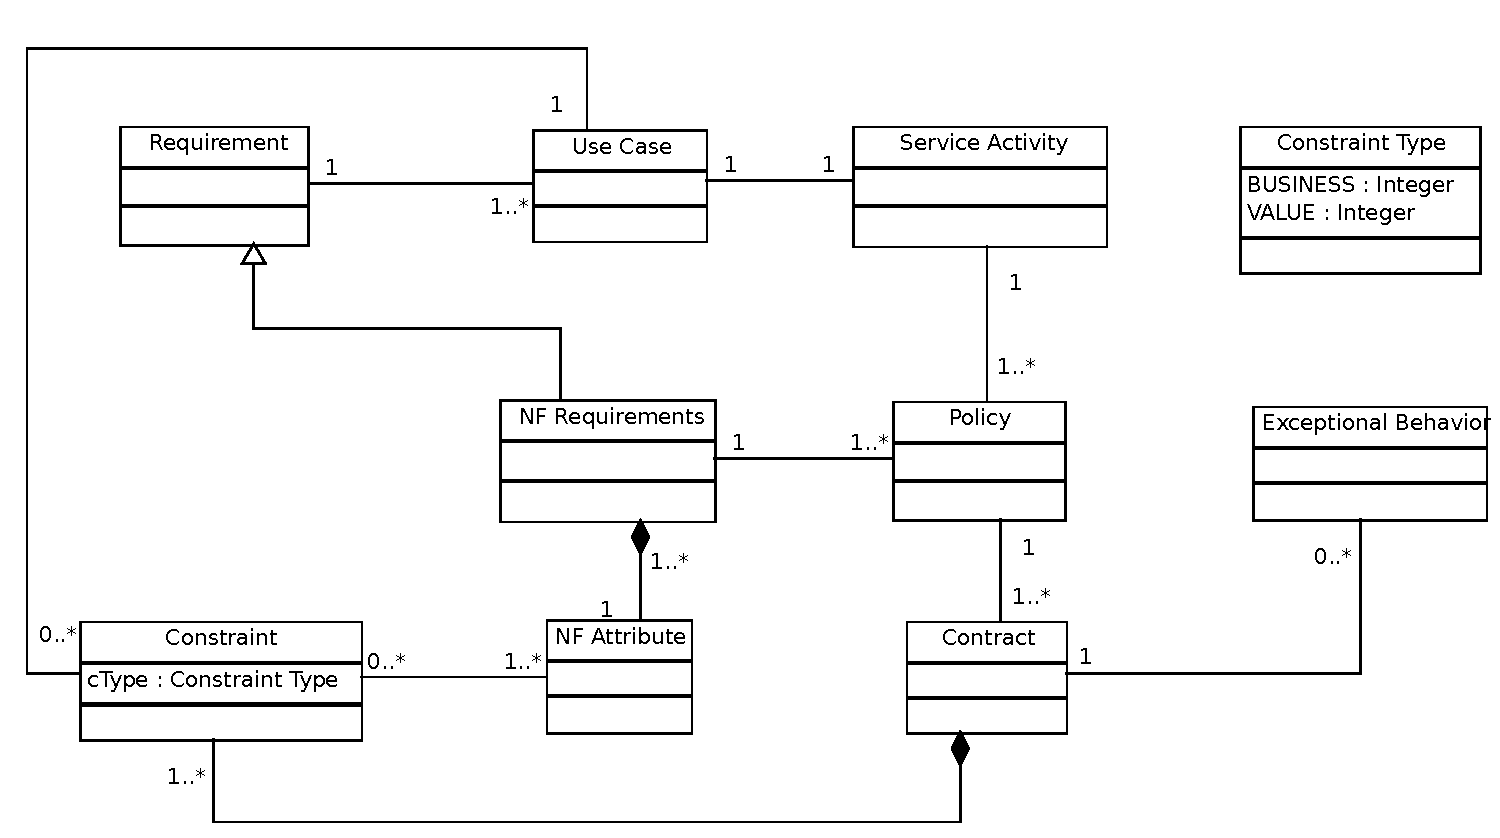
\includegraphics[width=0.99\textwidth]{chapters/state_ofthe_art/figs/contractModel.pdf}
\caption{Service-Based Non-Functional Requirement Model.}
\label{fig:NRFmodel} 
\end{figure}


A \textsc{Requirement}\footnote{We use this \textsc{Typeface} to refer to the
concepts of the model.}, whether functional or non-functional, can be
represented by one or more use cases. A use case represents a \texttt{Service Activity}. For example, a paying process can be modeled through the use cases
that represent withdrawal and deposit transactions and service provider
accounts. A payment process also requires the guarantee of a complete
transaction and data security. Thus several use cases model a single
requirement, and can be implemented as services.
% 
% A composite use case is a type of use case. This type of
% use case abstracts a more macro function, and may contain extra functions to be
% performed so that the process is complete. For example, to publish a song, you
% must choose which song you want to publish, , authenticate to twitter or facebook,
% so that the music you're listening is published. We consider this type of use
% case, a use case compound.
 
Each use case has \textit{business} or
\textit{value} constraints. \textit{Business constraints} are restrictions on
functions and how they may be implemented. The \textit{value constraints} are restrictions on
the service interface, expressing the desired values for input and output data.
Each constraint is associated with NFAs.

A \textsc{Contract} is a set of constraints for the same function. For example,
a contract for the payment operation. The constraints for payment are: (i) the
value amount should not be less than 10 euros and (ii) the user should always
receive a purchase confirmation by phone message. This restrictions are
grouped into a single contract for payment verification. 

% These constraints
% are also associated with non-functional attributes, e.g., reliability,
% transactions and data privacy card.
 
An \textsc{Exceptional Behavior} happens when a contract is not respected. When
this happens a new function is called or the process is stopped. For example, if
the bank does not authorize the payment, the system offers alternative forms
of payment such as PayPal.

Finally a \textsc{Policy} groups similar contracts. For example, security
contracts are grouped into a security policy and performance contracts are
grouped into a performance policy.


\subsection{NFR Classification}
\label{sec:nfr-classification}

Table \ref{tab:result04} shows the NFR classification we propose, organized
 as follows (by column): (i) the level of abstraction, (ii) the proper term for
 this kind of abstraction and (iii) possible values to be used. The rows
 represent the abstraction level for modeling the NFR. The highest level is the
 \textit{Business level}, the intermediary is the \textit{Service level}; and
 finally the \textit{System level}.  

\begin{table}[ht!]
\centering
%\scriptsize
\begin{tabular}{l|l|l}
  \hline 
  \hline
   \textbf{Modeling Level} & \textbf{\textit{Concept / Notation}} & \textbf{\textit{NFR / NFA}}  
   \\
  \hline
  \hline  
  Business Level & Constraint  & Business Constraint,    
 \\  
  &   & Value Constraint\\
  \hline   
   &  & Integrity, Transaction,  \\
   &  & Accessibility, \\
   &  & Cost, Time Constraint, \\
  Service Level & Contract & Platform, \\
   &  & Privacy, Authentication, \\
   &  & Resource, Capacity, \\
   &  &  Confidentiability 
   \\  \hline
   &  & Security, Performance,\\ 
   & & Interoperability, Scalability,\\
  System Level & Policy & Reliability, Usability,\\
   & & Availability\\
   \hline
  \hline  
\end{tabular}
\caption{Non-Functional Requirements Classification.}
\label{tab:result04}
\end{table} 



At the business modeling level, non-functional requirements are classified
into business restrictions. We have adopted, \textit{business} and \textit{value}
constraints to address the most abstract levels of restrictions in business
modeling. 

% We now present the proposed concepts for modeling NFR in all
% levels: business, service and system levels. We also  describe the
% meaning of each value presented in table \ref{tab:result04} the each specific
% level, starting at the business level. The values are:

% We have adopted this
% nomenclature for the fact that in business modeling level, the
% granularity is coarse. However, at this modeling level it is possible to
% identify if there are any restriction and if this restriction is over business
% functions or data. Thus


% For a business modeling it is
%   important to set out in detail the constraints that are likely to act as
%   limits on business activity.

%  limits on the values which it can represent. It is
%   often useful to be able to constrain the values which an element can take, perhaps to ensure that messages conform to business rules.
%   This concept describes how value constraints can be added to a simple type in
%   order to constrain the values of all elements based on it. 

\begin{itemize}
  \item \textbf{Business Constraint -} Represents rules for system
  development in terms of resource availability, interoperability, performance,
  dependencies, timescales.  Thus, \textit{Business Constraint}
  represents restrictions over business activities.
  \item \textbf{Value Constraint -} Defines valid subsets of values of a
  variable of a given type. In the context of services, value constraint are
  restrictions on the data on service calls (input and output values),
  expressing which range of values is allowed. This can be applied to
  authentication policies, access control, data integrity, cost of services, privacy, and other factors. 
\end{itemize}  

% % \subsubsection{Service NFR Definition:}    
% 
% The relationship between the concepts in business and service levels are
% presented below:
%  
% \begin{itemize}
%   \item Business constraint:
% 	\begin{itemize}
%   		\item Security; Performance; Availability; Interoperability; and Usability.
% 	\end{itemize}
%   \item Value constraint:
% 	\begin{itemize}
%   		\item Security; and Reliability.
% 	\end{itemize}
% \end{itemize}
  
% \subsubsection{System NFR Definition:}  

% Yeom et al. \cite{Yeom2006} describes some concepts for NFR in the system
% modeling. Some of these concepts is adapted for our context and proposal of NFR
% classification for web service modeling process. 


The following items describe the non-functional \correctingText{aspects} of the
service level. At the service level, the non-functional properties will be guaranteed upon
implementation of the service requirements.
  
\begin{itemize} 

  \item \textbf{Conformity -} Represents the degree at which a Web service
  function fulfills an application requirement.  
  
%   This is a factor to evaluate to which degree
%   the standard technology of web services are conformed. You can have functions
%   that perform this property, when necessary for customer's service.
%   
  \item \textbf{Time constraint -} This property can be associated to
  the execution time of a particular service. This property is related
  to services performance and availability.  
  \item \textbf{Capacity -} Represents the degree at which a service can
  process a given volume of data or requests.
  \item \textbf{Cost -} Represents the cost to run a service. It can be in
   time, bandwidth and money.
  \item \textbf{Privacy -}  The challenge in data privacy is to share
  data while protecting personally identifiable information. Privacy of
  Web services is the ability of the service must have to preserve the data and
  user information. 
  \item \textbf{Authentication -} Represents the process of making sure
  that the person who is asking to use the web service is really the person that
  they claim to be. 
  \item \textbf{Accessibility -} Represents the quality aspect of a web
  service related with the degree to which it is capable of serving a
 request. 
  \item \textbf{Access control -} Refers to exerting control over who can
  interact with a resource, \textit{e.g.} computer-based information system, a
  service or a database \cite{Adiba:1981}. 
  \item \textbf{Confidentiability -} Confidentiality ensures that
  information is not accessed by unauthorized people. The private data is
  accessed only by authorized users. 
  \item \textbf{Integrity -} \correctingText{Define the security attributes of the system,
  restricting access to features or data to certain users and protecting the
  privacy of data entered into the software \cite{Greene2005}. It also represents
  the ability of the web service to maintain the correctness of the interaction which is
  ensured by the proper execution of a web service transaction.}
   \item \textbf{Transaction -} A transaction is a unit of work performed
  to maintain a data integrity in a known and consistent state \cite{Adiba:1981}.
  \item \textbf{Resource -} A resource is any physical or virtual
  component of limited availability within a computer or information management
  system. Computer resources include means for receiving, processing, notifying,
  transmitting and storing data \cite{Adiba:1981}. 
 \item \newText{\textbf{Platform -} Web services platform management is the
    management of the platform on which a web service is installed and provided. It is
 available as long as such a platform is with the standard management interface
 \cite{Yeom2006}.}
\end{itemize}  


The \correctingText{non-functional aspects, expressed as \textit{Contracts},}
at the system level represent the behaviour of the workflow. Following,
the properties we considered important for this level are defined.

\begin{itemize}
  \item \textbf{Usability -} ISO defines usability as ``\textit{The extent to which a
  product can be used by specified users to achieve specified goals with
  effectiveness, efficiency, and satisfaction in a specified context of use}''.
  \newText{Ease-of-use requirements address the factors that constitute the capacity
  of the software to be understood, learned, and used by its intended users
  \cite{Greene2005}.} In the context of services, usability can mean how
  efficient and easy to access a service is and whether it satisfies the needs of those who are invoking this service.
  \item \textbf{Interoperability -} \correctingText{Is a property referring to
  the ability of diverse systems to work together. If two or
  more systems are capable of communicating and exchanging data, they are
  exhibiting syntactic interoperability \cite{MylopoulosBook99}.} According to
  ISO interoperability is defined as ``\textit{The capability to communicate, execute functions, or transfer
  data among various functional units in a manner that requires the user to have
  little or no knowledge of the unique characteristics of those units}''. In the
  context of services, interoperability can mean that the services have capacity
  to communicate with each other.  
%   The term
%   \textit{choreography} can simplify the understanding of interoperability
%   between services. 
\item \textbf{Scalability -} \newText{Software that is scalable has the ability to
handle a wide variety of system configuration sizes. The nonfunctional requirements should specify the
ways in which the system may be expected to scale up \cite{Greene2005}.}
  \item \textbf{Reliability -} The concept of reliability has different
  applications in different areas. Applied to web services, reliability is the
  ability of the service to execute correctly the methods it exports. It is also
  important that the data presented are consistent with the expected result.
  \newText{Reliability specifies the capability of the software to maintain its
  performance over time. Unreliable software fails frequently, and certain tasks
  are more sensitive to failure \cite{Greene2005}.}  
  \item \textbf{Availability -}  \newText{A system's availability, or uptime, is the
  amount of time that it is operational and available for use
  \cite{Greene2005}.} Is the proportion of time a service is in a functioning condition. This is often described as a mission capable rate. Availability of web services, is the probability of a service call 
  to be successful, given a specific time. 
  \item \textbf{Performance -} In the context of web services, performance is how fast the service can be
  executed in accordance with the needs of the user. \newText{The performance
  constraints specify the timing characteristics of the software
  \cite{Greene2005}.}
  \item \textbf{Security -} Represents protecting information and
  information systems from unauthorized access, use, disclosure, disruption,
  modification, perusal, inspection, recording or destruction \cite{MylopoulosBook99}.  
%   Security as a form of protection are structures and
%   processes that provide or improve security as a condition. Security of data is
%   the means of ensuring that data is kept safe from corruption and that access to it
%   is suitably controlled. But security also m
\end{itemize}


The relationship between non-functional requirements and attributes help to
identify groups of restrictions and contracts to develop specific policies. The
level of service shows non-functional requirements, and system level presents a
finer granularity, describing the non-functional attributes. Thus, a set of
contracts that are related to the same attribute form specific policies for the
system. The relationship between the concepts in business, service and system
levels are presented in figure \ref{fig:nfr-relationship}.

\begin{figure}[ht!]  
\centering  
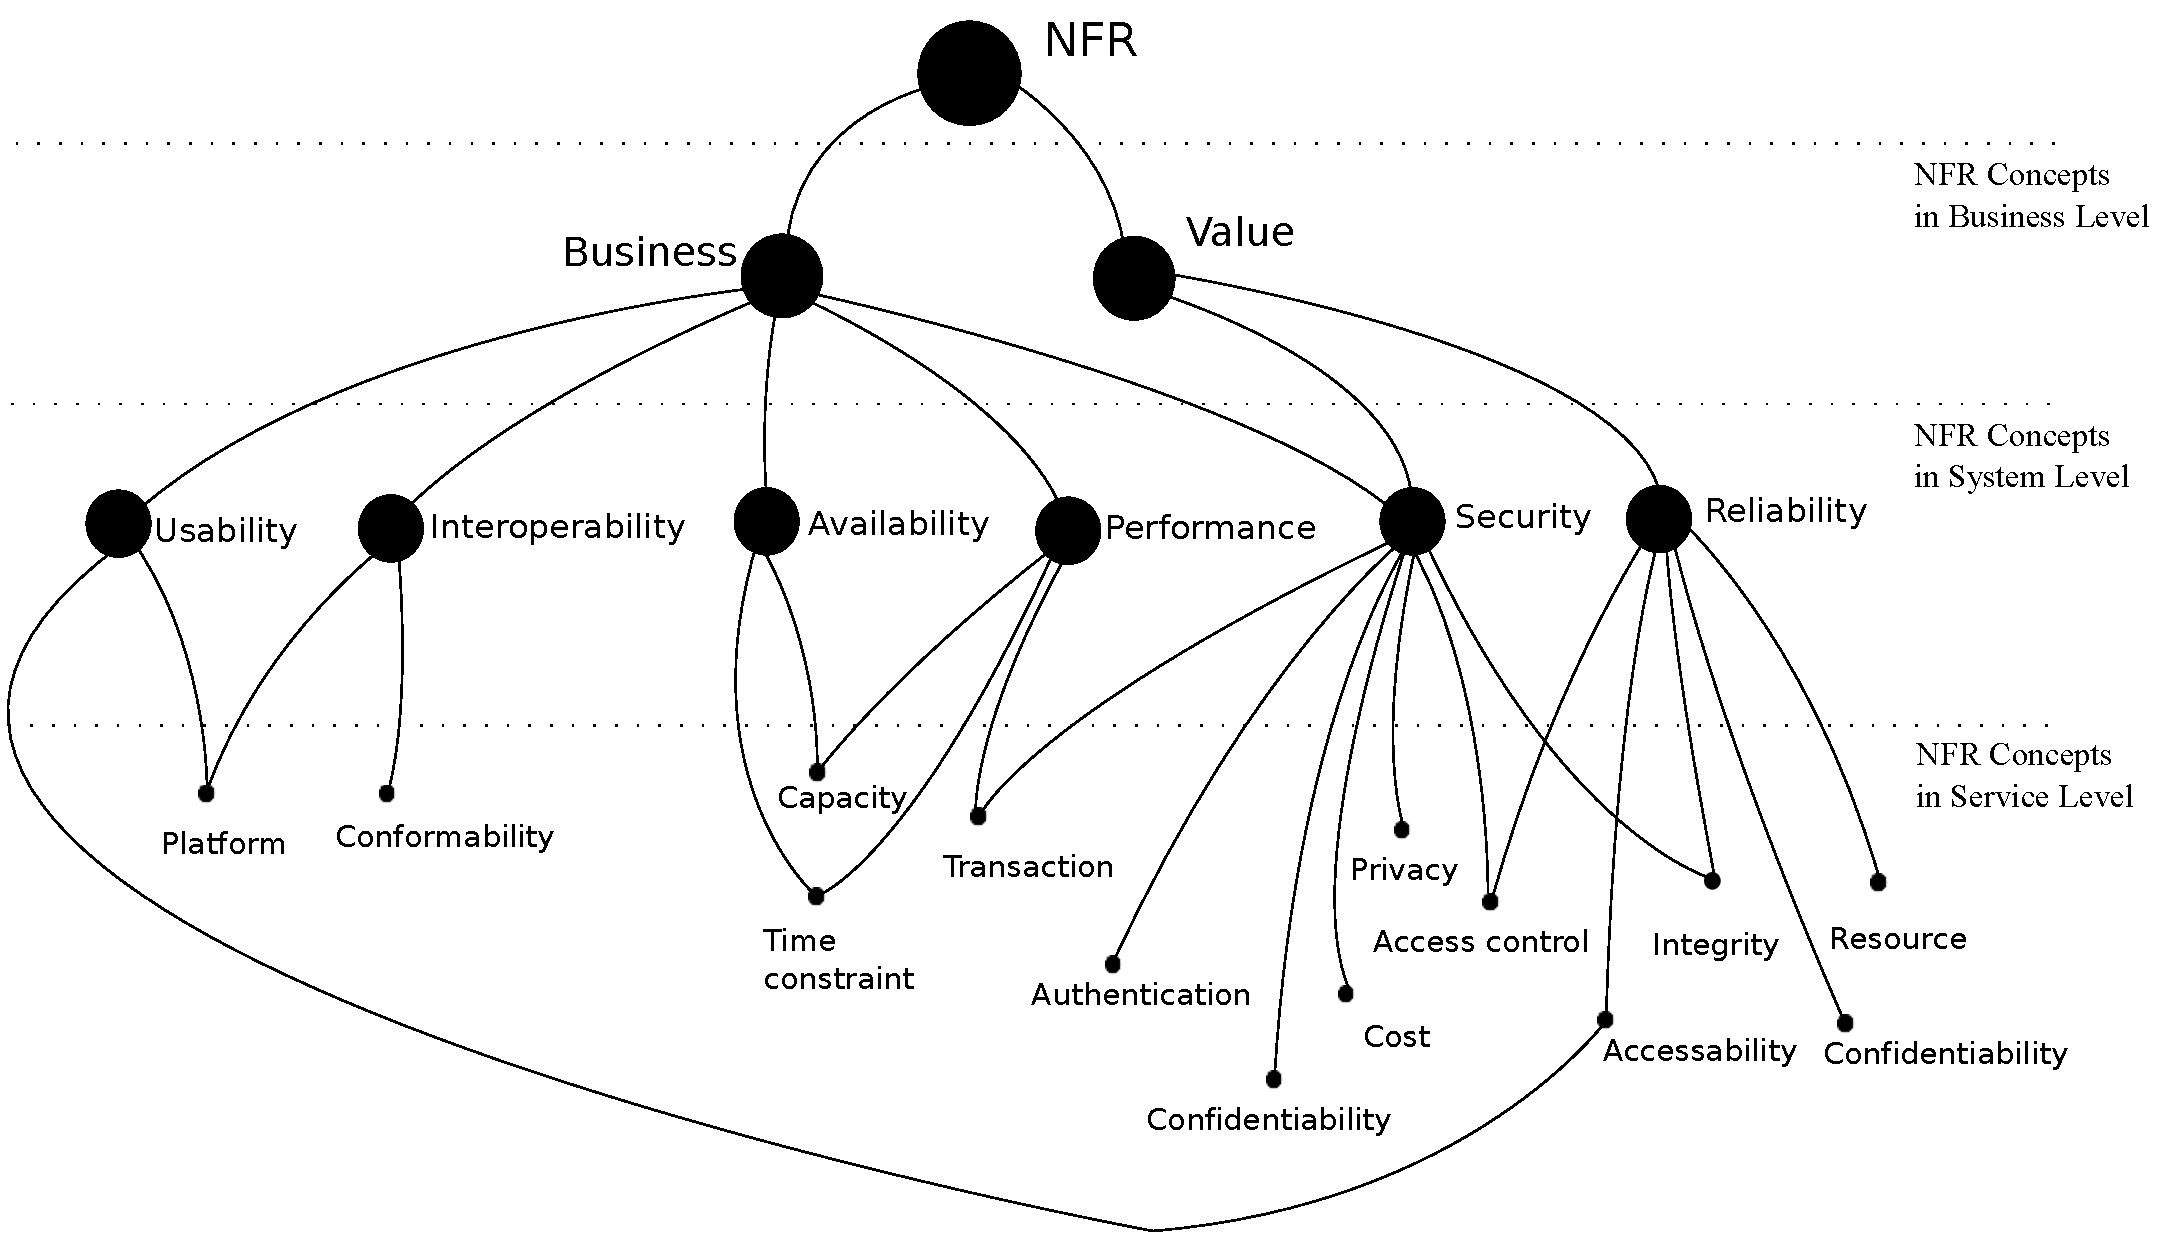
\includegraphics[width=0.99\textwidth]{chapters/state_ofthe_art/figs/nfrRelationship.pdf}
\caption{Relationship of the NFR Concepts.}
\label{fig:nfr-relationship}   
\end{figure}    
 
% \begin{itemize}
%   \item Security:
% 	\begin{itemize}
%   		\item Access control; Transaction; Privacy; Cost; Authentication;
%   		Integrity; and Confidentiability.
% 	\end{itemize}
%   \item Performance:
% 	\begin{itemize}
%   		\item Time constraint; Capacity; and Transaction.
% 	\end{itemize}
% 	\item Availability:
% 	\begin{itemize}
%   		\item Capacity; and Time constraint.
% 	\end{itemize}
% 	\item Interoperability:
% 	\begin{itemize}
%   		\item Conformability; and Platform.
% 	\end{itemize}
% 	\item Usability: 
% 	\begin{itemize}
%   		\item Accessibility; and Platform.
% 	\end{itemize}
% 	\item Reliability:
% 	\begin{itemize}
%   		\item Access control; Confidentiability; Accessibility; Integrity; and
%   		Resource.
% 	\end{itemize}
% \end{itemize}


% \begin{figure} 
% \centering
% \includegraphics[width=.7\textwidth]{figs/PiSODM.png}
% \caption{Non-functional requirements for PiSOD-M Methodology.}
% \label{fig:PiSODM}
% \end{figure} 

% Considering the structure and the concepts (figure \ref{fig:PiSODM}) of PiSOD-M,
% the non-functional requirements will being refined from CIM level to PSM level,
% being observed the specific areas of each application.

In our work we adopt \textit{security, performance, availability,
interoperability, usability} and \textit{reliability} as NFRs, and we consider
as NFAs \textit{access control, time constraint, privacy, accessibility},
\textit{etc}. These terms and proposed values will be used in chapter
 \ref{chapter:methodology}. The methodology that will be presented in the next
 chapter uses this nomenclature for modeling the non-functional requirements in
 the development of service-oriented applications.

%********************************************************************************************************* 
\section{Conclusions}
\label{sec:stateofart_conclusion}
%*********************************************************************************************************


This chapter presented a review of related approaches for the
service-oriented development of applications. We consider two important
topics in our analysis: \textit{(i)} non-functional requirements and
\textit{(ii)} methodologies for service-based development. The revised methods
were grouped according to their characteristics, and analyzed their context
of application.
 

We reviewed existing methodologies for service-based development. We
analyze other general aspects of these methodologies as their
development paradigm, use of the UML and formalism, and whether the method
considered an MDA-based development or not. In this case we have studied the main techniques
and methods proposed for modelling non-functional requirements,
business process and web service composition.
% 
% In general, after reviewing the current research works related
% with the problem of service-oriented development, we could obtain
% some conclusion. 

To the best of our knowledge, there are no proposals that define a
service-oriented approach for the whole development of systems, considering
non-functional requirements. Although many efforts have been made to support the new
technological proposals for the Web such as web services, in general, these
methodologies focus their processes on traditional software
engineering approaches, with emphasis on the functional aspects of the
application.

The comparative study of such methodological approaches for service development
is the basis for the design decisions of the method we propose in
this work.
 
% \begin{figure}  [ht!]
% \centering  
% 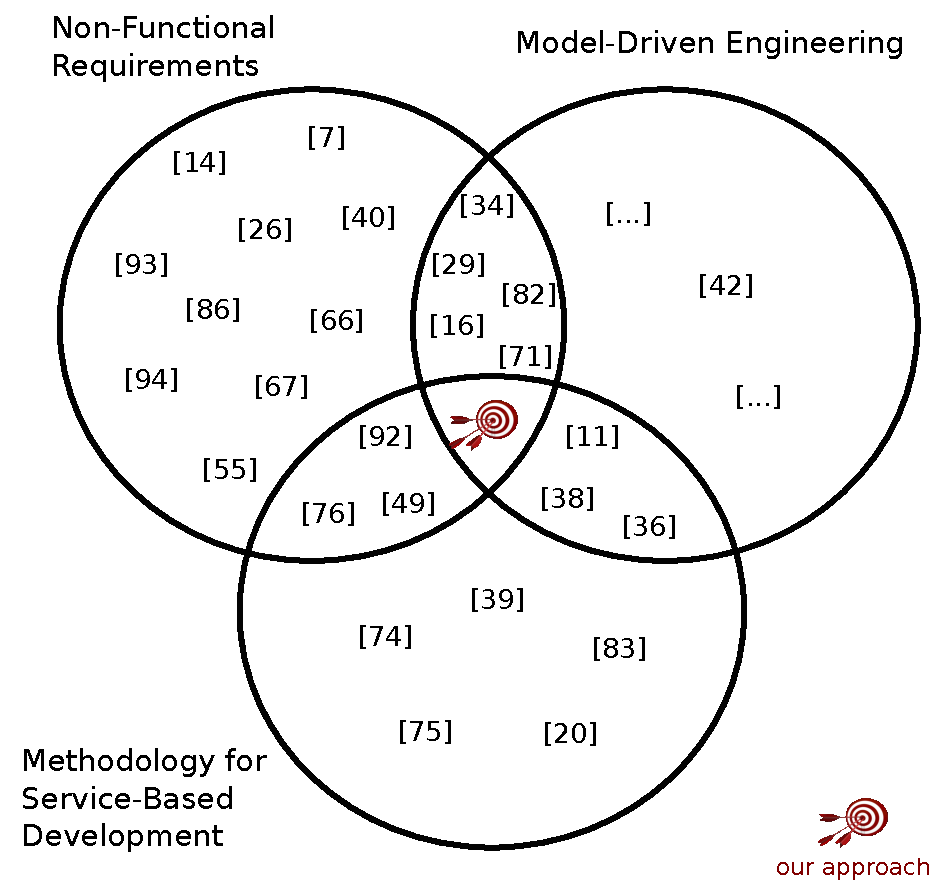
\includegraphics[width=0.6\textwidth]{chapters/state_ofthe_art/figs/ourApproach.pdf}
% \caption{Related Works Analysis.}
% \label{fig:ourApproach}   
% \end{figure}  
  
 
% Figure \ref{fig:ourApproach} presents an overview of related work and their
% specific areas. 
The analysis helped us identify a gap for improving the development of service-based
applications. Our approach targets to deal with characteristics of the 3
areas\footnote{(i) Non-Functional Requirements; (ii) Methodology for Service-Based Development;
and (iii) Model-Driven Engineering} in order to propose a methodology for
developing service-based applications considering non-functional aspects.

% to minimize the problem of do not have a
% methodology for developing service-based applications that consider non-functional aspects.

Our work addresses the development of reliable service-based applications that
uses services and non-functional aspects.

\newText{
Similar to approaches such as WS-*, our work targets the specification and programming of service-oriented  applications,
including its non-functional aspects (i.e., atomicity, security, performance,
persistence). Our work
specifies \textit{policies} for modeling the non-functional requirements of a service composition in an orthogonal way,
\textit{i.e} separating the specification of non-functional requirements from
the main functionalities of the application. This is interesting because once  the policies for a
given application have been defined they can be reused and/or specialized for another application
with similar requirements.


The main goal of the methodology we propose in this thesis is to provide a way
for supporting the development of service-oriented  applications in the presence of non-functional
properties. The use of the WS-* standards
supposes that non-functional requirements are implemented according to the
knowledge that a programmer has of a specific application requirements, without
deriving them according to a methodology, thus leading to \textit{ad-hoc} solutions
that can be difficult to reuse. The goal is to provide a way for supporting the
development of service-oriented  applications in the presence of non-functional
properties. 
   
 
The methodology that will be presented provides a model-driven structure that
encompasses concepts related with service-oriented development and
non-functional properties (modelled as \textit{Contracts} and
\textit{Policies}). The methodology provides a set of concepts, steps and
transformations to develop service-oriented applications.  
 
Given that our approach is MDA-based, it allows the specification
of service compositions as an abstract model, which may be realized as a
concrete implementation (program). 
}



In the following chapters we describe a service-based  methodology that
we propose and that focusses on non-functional aspects description and modeling.
For this, we use model-based development (MDD) and the classification of non-functional requirements
described in this chapter, as well as the meta-model with NFR notation.     





% \begin{sidewaystable}[h]\caption{Performance After Post Filtering} % title name of the table\centering % centering table\begin{tabular}{l c c rrrrrrr} % creating 10 columns\hline\hline % inserting double-lineAudio &Audibility & Decision &\multicolumn{7}{c}{Sum of Extracted Bits}\\ [0.5ex]\hline % inserts single-line% Entering 1
% st
% row& &soft &1 & $-1$ & 1 & 1 & $-1$ & $-1$ & 1 \\[-1ex]\raisebox{1.5ex}{Police} & \raisebox{1.5ex}{5}&hard& 2 & $-4$ & 4 & 4 & $-2$ & $-4$ & 4 \\[1ex]% Entering 2
% nd
% row& &soft & 1 & $-1$ & 1 & 1 & $-1$ & $-1$ & 1 \\[-1ex]\raisebox{1.5ex}{Beethoven} & \raisebox{1.5ex}{5}& hard&8 & $-8$ & 2 & 8 & $-8$ & $-8$ & 6 \\[1ex]% Entering 3
% rd
% row& &soft & 1 & $-1$ & 1 & 1 & $-1$ & $-1$ & 1 \\[-1ex]\raisebox{1.5ex}{Metallica} & \raisebox{1.5ex}{5}& hard&4 & $-8$ & 8 & 4 & $-8$ & $-8$ & 8 \\[1ex]% [1ex] adds vertical space\hline % inserts single-line\end{tabular}\label{tab:LPer}\end{sidewaystable}
